\documentclass{report}
\usepackage{amsmath,amsfonts,amsthm}
\usepackage{authblk}
\usepackage[T1]{fontenc}
\usepackage{graphicx}
\usepackage[utf8]{inputenc}
\usepackage[framemethod=tikz]{mdframed}
\usepackage{natbib}
\usepackage{subcaption}
\usepackage{tikz}
\usepackage{xcolor}

\usepackage{hyperref}

\definecolor{blue}{RGB}{38,139,210}
\definecolor{cyan}{RGB}{42,161,152}
\definecolor{red}{RGB}{220,50,47}
\definecolor{base01}{RGB}{88,110,117}
\definecolor{base02}{RGB}{7,54,66}
\definecolor{base03}{RGB}{0,43,54}

\usetikzlibrary{calc,shapes,positioning}

\newcommand{\todo}[1]{\textcolor{red}{TODO: #1}}

\newtheorem{prop}{Property}
\providecommand*{\propautorefname}{Property}
\surroundwithmdframed[
    topline=false,
    bottomline=false,
    middlelinewidth=0.5pt,
    linecolor=base01,
    roundcorner=5pt,
    innertopmargin=0pt,
    leftmargin=15pt,
    rightmargin=15pt,
    nobreak=true,
]{prop}

\setcounter{MaxMatrixCols}{16}

\title{A guide to convolution arithmetic for deep learning}
\author[*]{Vincent Dumoulin\thanks{dumouliv@iro.umontreal.ca}}
\author[*]{Francesco Visin\thanks{fvisin@gmail.com}}
\affil[*]{MILA, Universit\'{e} de Montr\'{e}al}
\date{\today}

\begin{document}

\maketitle

\chapter{Introduction}

Deep convolutional neural networks (CNNs) have been at the heart of spectacular
advances in deep learning. Although CNNs have been used as early as the nineties
\citep{lecun1998gradient} to solve character recognition tasks, their current
widespread application is due to much more recent work, when a deep CNN was used
to beat state-of-the-art in the ImageNet image classification challenge
\citep{krizhevsky2012imagenet}.

Convolutional neural networks therefore constitute a very useful tool for
machine learning practitioners. However, learning to use CNNs for the first time
is generally an intimidating experience. A convolutional layer's output shape is
affected by the shape of its input as well as the choice of kernel shape, zero
padding and strides, and the relationship between these properties is not
trivial to infer. This contrasts with fully-connected layers, whose output size
is independent of its input size.

Additionally, so-called transposed convolutional layers (also known as
fractionally strided convolutional layers) have been employed in more and more
work as of late, and their relationship with convolutional layers has been
explained with various degrees of clarity.

This guide's objective is twofold:

\begin{enumerate}
    \item Explain the relationship between convolutional layers and transposed
        convolutional layers.
    \item Provide an intuitive understanding of the relationship between input
        shape, kernel shape, zero padding, strides and output shape in
        convolutional layers and transposed convolutional layers.
\end{enumerate}

\section{Discrete convolutions}

The bread and butter of neural networks is affine transformations: a vector is
received as input and is multiplied with a matrix to produce an output (to which
a bias vector is usually added before passing the result through a
nonlinearity). This is applicable to any type of input, be it an image, a sound
clip or an unordered collection of features: their representation can always be
flattened into a vector before the transformation.

In the case of images and sound clips, there is an ordering (spatial or
temporal) being thrown away when they are flattened. This information may prove
very handy in solving some tasks, like computer vision and speech recognition.

These sorts of inputs share important properties:

\begin{itemize}
    \item They are stored as multi-dimensional arrays.
    \item They feature one or more axes for which ordering matters (e.g. width
        and height axes for an image, time axis for a sound clip).
    \item One axis, called the channel axis, is used to access different views
        of the data (e.g. the red, green and blue channels of a color image, or
        the left and right channels of a stereo audio track).
\end{itemize}

A discrete convolution is a linear transformation that is sparse (only a few
input units contribute to a given output unit) and reuses parameters (the same
transformation is applied to multiple locations in the input).

\autoref{fig:numerical_no_padding_no_strides} provides an example of a discrete
convolution. The blue grid is called the input {\em feature map}\footnote{
    What was referred to earlier as {\em channels} is a name for the {\em
    feature maps} of input data.}.
A {\em kernel} (dark blue) of value

\begin{equation}
\begin{pmatrix}
    0 & 1 & 2 \\
    2 & 2 & 0 \\
    0 & 1 & 2
\end{pmatrix}
\end{equation}

slides across the input feature map. At each location, the product between the
kernel elements and the overlapped input elements is computed and the results
are summed up to obtain the corresponding output {\em feature map}
value\footnote{
    While there is a distinction between convolution and cross-correlation from
    a signal processing perspective, the two become interchangeable when the
    kernel is learned. For the sake of simplicity and to stay consistent with
    most of the machine learning litterature, the term {\em convolution}
    will be used in this guide.}.

If there are multiple input feature maps, each input feature map is convolved
with a distinct kernel, and the resulting feature maps are summed up elementwise
to produce the output feature map. The procedure can be repeated using different
kernels to form as many output feature maps as desired.

The convolution presented in \autoref{fig:numerical_no_padding_no_strides} is an
instance of a 2-D convolution, but it can be generalized to N-D convolutions.
For instance, in a 3-D convolution, the kernel would be a {\em cuboid} and would
slide across the height, width and depth of the input feature map.

The collection of kernels defining a discrete convolution has a shape
corresponding to some permutation of $(n, m, k_1, \ldots, k_N)$, where

\begin{equation}
\begin{split}
    n &\equiv \text{number of output feature maps},\\
    m &\equiv \text{number of input feature maps},\\
    k_j &\equiv \text{kernel size along axis $j$}.
\end{split}
\end{equation}

The following properties affect the output size $o_j$ of a convolutional layer
along axis $j$:

\begin{itemize}
    \item $i_j$: input size along axis $j$,
    \item $k_j$: kernel size along axis $j$,
    \item $s_j$: stride (distance between two consecutive positions of the
        kernel) along axis $j$,
    \item $p_j$: zero-padding (number of zeros concatenated at the beginning and
        at the end of an axis) along axis $j$.
\end{itemize}

For instance, \autoref{fig:numerical_padding_strides} shows a $3 \times 3$
kernel applied to a $5 \times 5$ input padded with a $1 \times 1$ border of
zeros using $2 \times 2$ strides.

The analysis of the relationship between these parameters is simplified by the
fact that they don't interact across axes, i.e. choices of kernel size, stride
and zero padding along axis $j$ only affect the output size of axis $j$.

Because of this, the guide will concentrate on 2-D convolutional layers acting
on square inputs, and the kernel size, stride and zero-padding will always be
the same along both axes.

\begin{figure}[p]
    \centering
    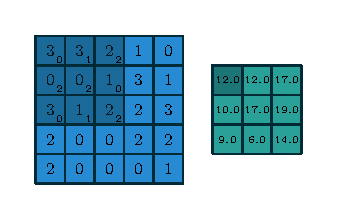
\includegraphics[width=0.32\textwidth]{pdf/numerical_no_padding_no_strides_00.pdf}
    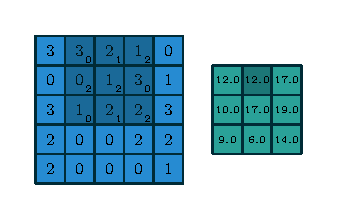
\includegraphics[width=0.32\textwidth]{pdf/numerical_no_padding_no_strides_01.pdf}
    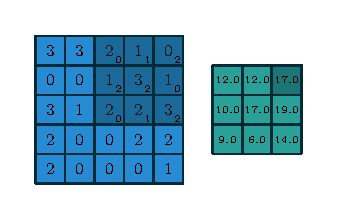
\includegraphics[width=0.32\textwidth]{pdf/numerical_no_padding_no_strides_02.pdf}
    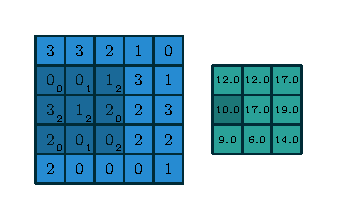
\includegraphics[width=0.32\textwidth]{pdf/numerical_no_padding_no_strides_03.pdf}
    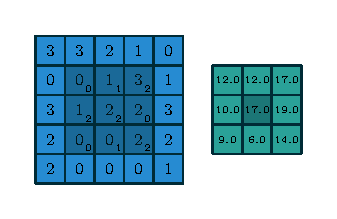
\includegraphics[width=0.32\textwidth]{pdf/numerical_no_padding_no_strides_04.pdf}
    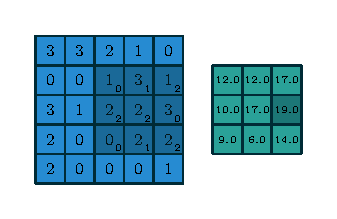
\includegraphics[width=0.32\textwidth]{pdf/numerical_no_padding_no_strides_05.pdf}
    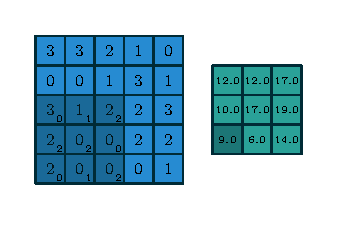
\includegraphics[width=0.32\textwidth]{pdf/numerical_no_padding_no_strides_06.pdf}
    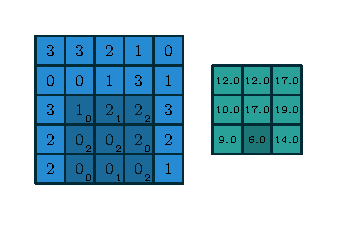
\includegraphics[width=0.32\textwidth]{pdf/numerical_no_padding_no_strides_07.pdf}
    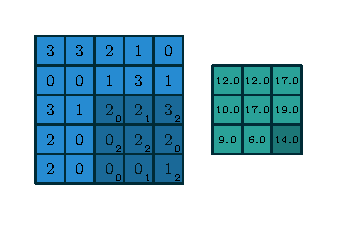
\includegraphics[width=0.32\textwidth]{pdf/numerical_no_padding_no_strides_08.pdf}
    \caption{\label{fig:numerical_no_padding_no_strides} Computing three output
        values of a discrete convolution.}
\end{figure}

\begin{figure}[p]
    \centering
    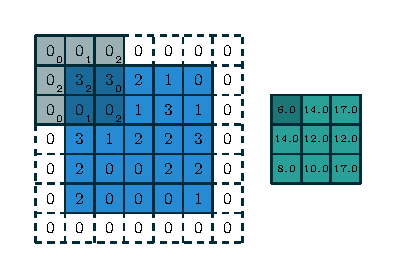
\includegraphics[width=0.32\textwidth]{pdf/numerical_padding_strides_00.pdf}
    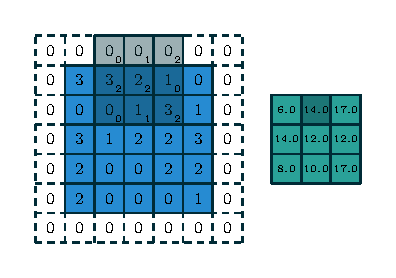
\includegraphics[width=0.32\textwidth]{pdf/numerical_padding_strides_01.pdf}
    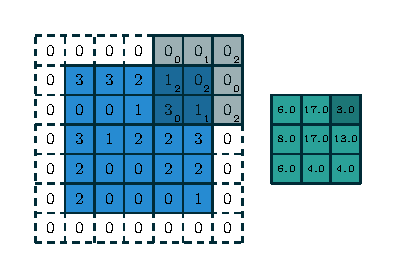
\includegraphics[width=0.32\textwidth]{pdf/numerical_padding_strides_02.pdf}
    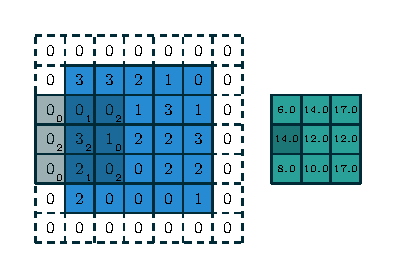
\includegraphics[width=0.32\textwidth]{pdf/numerical_padding_strides_03.pdf}
    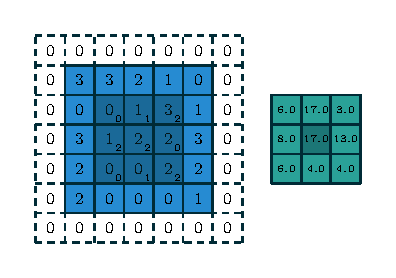
\includegraphics[width=0.32\textwidth]{pdf/numerical_padding_strides_04.pdf}
    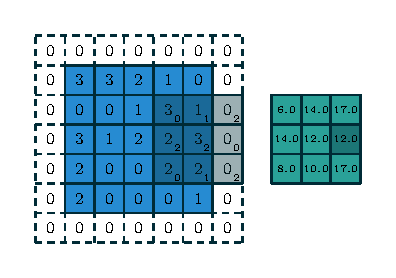
\includegraphics[width=0.32\textwidth]{pdf/numerical_padding_strides_05.pdf}
    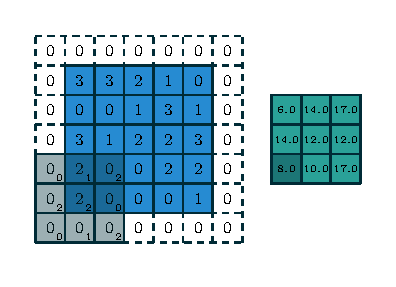
\includegraphics[width=0.32\textwidth]{pdf/numerical_padding_strides_06.pdf}
    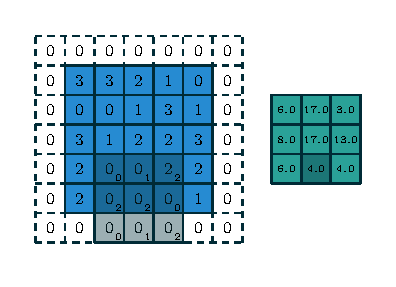
\includegraphics[width=0.32\textwidth]{pdf/numerical_padding_strides_07.pdf}
    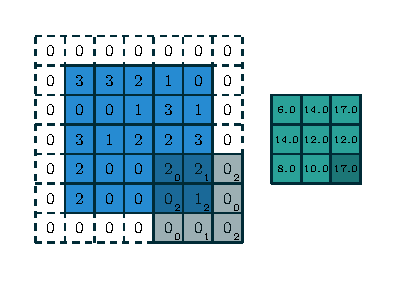
\includegraphics[width=0.32\textwidth]{pdf/numerical_padding_strides_08.pdf}
    \caption{\label{fig:numerical_padding_strides} Computing three output values
        of a discrete convolution for $N = 2$, $i_1 = i_2 = 5$, $k_1 = k_2 = 3$,
        $s_1 = s_2 = 2$, and $p_1 = p_2 = 1$.}
\end{figure}

\chapter{Convolution arithmetic}

\section{No zero-padding, unit strides}

The simplest case to analyze is when a kernel just slides across the input (i.e.
$s = 1$ and $p = 0$). \autoref{fig:no_padding_no_strides} provides an example
for $i = 4$ and $k = 3$.

One way of defining the output size is by the number of possible placements of
the kernel on the input. Consider the width axis: the left side of the kernel
starts at the left side of the input, and the kernel slides by steps of one
until its right side touches the right side of the input. The size of the output
is equal to the number of steps made, plus one, accounting for the initial
position of the kernel (\autoref{fig:no_padding_no_strides_explained}). The same
logic applies for the height axis.

From this, the following property is inferred:

\begin{prop}\label{prop:no_padding_no_strides}
For $i$, $k$, $s = 1$ and $p = 0$,
\begin{equation*}
    o = (i - k) + 1.
\end{equation*}
\end{prop}

\section{Zero-padding, unit strides}

To factor in zero-padding (i.e. only restricting that $s = 0$), consider its
effect on the effective input size. \autoref{fig:arbitrary_padding_no_strides}
provides an example for $i = 5$, $k = 4$ and $p = 2$.

Noting that padding with $p$ zeros changes the effective input size from $i$ to
$i + 2p$, \autoref{prop:no_padding_no_strides} is used to infer the following
property:

\begin{prop}\label{prop:arbitrary_padding_no_strides}
For $i$, $k$, $s = 1$ and $p$,
\begin{equation*}
    o = (i - k) + 2p + 1.
\end{equation*}
\end{prop}

Two specific instances of zero padding are used quite extensively in practice
because of their respective properties.

\subsection{Half padding}

Having the output size be the same as the input size can be a desireable
property:

\begin{prop}\label{prop:same_padding_no_strides}
If $k$ is odd ($k = 2n + 1, \quad n \in \mathbb{N}$), and for $i$, $s = 1$ and
$p = \lfloor k / 2 \rfloor = n$,
\begin{equation*}
\begin{split}
    o &= i + 2 \lfloor k / 2 \rfloor - (k - 1) \\
      &= i + 2n - 2n \\
      &= i.
\end{split}
\end{equation*}
\end{prop}

This is sometimes referred to as {\em half} (or {\em same}) padding.
\autoref{fig:same_padding_no_strides} provides an example for $i = 5$, $k = 3$
and (therefore) $p = 1$.

\subsection{Full padding}

While convolving a kernel generally {\em decreases} the output size with respect
to the input size, sometimes the opposite is required:

\begin{prop}\label{prop:full_padding_no_strides}
If $p = k - 1$, and for $i$, $k$ and $s = 1$,
\begin{equation*}
\begin{split}
    o &= i + 2(k - 1) - (k - 1) \\
      &= i + (k - 1).
\end{split}
\end{equation*}
\end{prop}

This is sometimes referred to as {\em full} padding, because in this setting
every element of the kernel is superimposed on every element of the input
feature map. \autoref{fig:full_padding_no_strides} provides an example for $i =
5$, $k = 3$ and (therefore) $p = 2$.

\section{No zero-padding, non-unit strides}

So far, all properties derived only apply for unit-strided convolutions.
Incorporating non-unit strides requires another inference leap. To facilitate
the analysis, let's momentarily ignore zero-padding (i.e.  $s > 1$ and $p = 0$).
\autoref{fig:no_padding_strides} provides an example for $i = 5$, $k = 3$ and $s
= 2$.

Once again, the output size is defined in terms of the number of possible
placements of the kernel on the input. Consider the width axis: the left side of
the kernel starts at the left side of the input, but this time the kernel slides
by steps of $s$ until its right side touches the right side of the input. The
size of the output is equal to the number of steps made, plus one, accounting
for the initial position of the kernel
(\autoref{fig:no_padding_strides_explained}). The same logic applies for the
height axis.

From this, the following property is inferred:

\begin{prop}\label{prop:no_padding_strides}
For $i$, $k$, $p = 0$ and $s$,
\begin{equation*}
    o = \left\lfloor \frac{i - k}{s} \right\rfloor + 1.
\end{equation*}
\end{prop}

The floor function accounts for the fact that sometimes the last possible step
does {\em not} coincide with the kernel reaching the end of the input, i.e.
some input units are left out (see \autoref{fig:padding_strides_odd} for an
example of such a case).

\section{Zero-padding, non-unit strides}

The most general case (convolving over a zero-padded input using non-unit
strides) is analyzed by applying \autoref{prop:no_padding_strides} on an
effective input of size $i + 2p$, just as was done for
\autoref{prop:arbitrary_padding_no_strides}:

\begin{prop}\label{prop:padding_strides}
For $i$, $k$, $p$ and $s$,
\begin{equation*}
    o = \left\lfloor \frac{i + 2p - k}{s} \right\rfloor + 1.
\end{equation*}
\end{prop}

\autoref{fig:padding_strides} provides an example for $i = 5$, $k = 3$, $s = 2$
and $p = 1$.

As was noted for \autoref{prop:no_padding_strides}, the floor function means
that in some cases a convolution will produce the same output size for multiple
input sizes.

More specifically, if $i + 2p - k$ is a multiple of $s$, then any input size $j
= i + a, \quad a \in \{0,\ldots,s - 1\}$ will produce the same output size. Note
that this ambiguity applies only for $s > 1$.

\autoref{fig:padding_strides_odd} provides an example for $i = 6$, $k = 3$, $s =
2$ and $p = 1$. Despite having different input sizes, the convolutions presented
in \autoref{fig:padding_strides} and \autoref{fig:padding_strides_odd} share the
same output size.

While this doesn't affect the analysis for {\em convolutions}, this will
complicate the analysis in the case of {\em transposed convolutions}.

\begin{figure}[p]
    \centering
    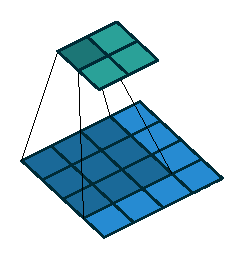
\includegraphics[width=0.24\textwidth]{pdf/no_padding_no_strides_00.pdf}
    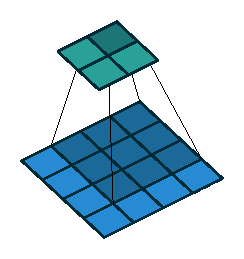
\includegraphics[width=0.24\textwidth]{pdf/no_padding_no_strides_01.pdf}
    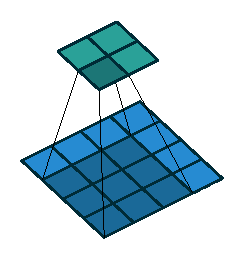
\includegraphics[width=0.24\textwidth]{pdf/no_padding_no_strides_02.pdf}
    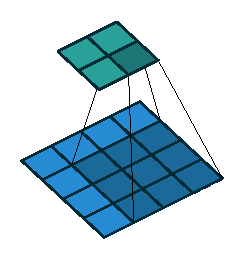
\includegraphics[width=0.24\textwidth]{pdf/no_padding_no_strides_03.pdf}
    \caption{\label{fig:no_padding_no_strides} Convolving a $3 \times 3$ kernel
        over a $4 \times 4$ input using unit strides (i.e. $i = 4$, $k = 3$,
        $s = 1$ and $p = 0$).}
\end{figure}

\begin{figure}[p]
    \centering
    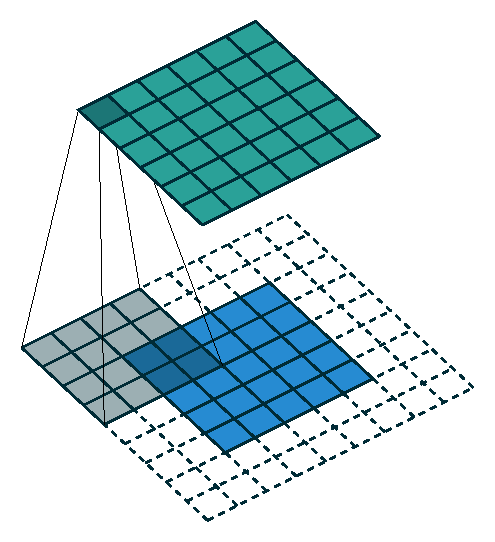
\includegraphics[width=0.24\textwidth]{pdf/arbitrary_padding_no_strides_00.pdf}
    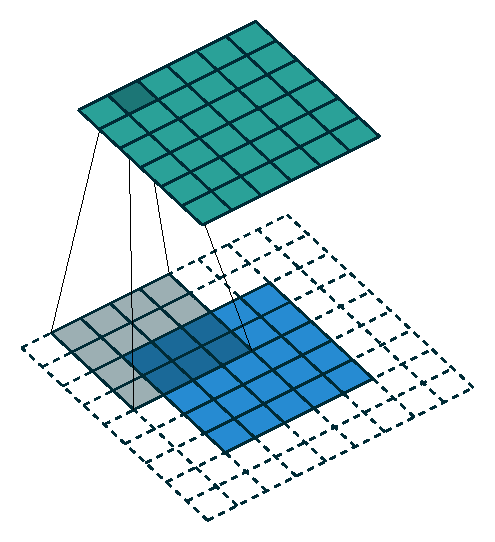
\includegraphics[width=0.24\textwidth]{pdf/arbitrary_padding_no_strides_01.pdf}
    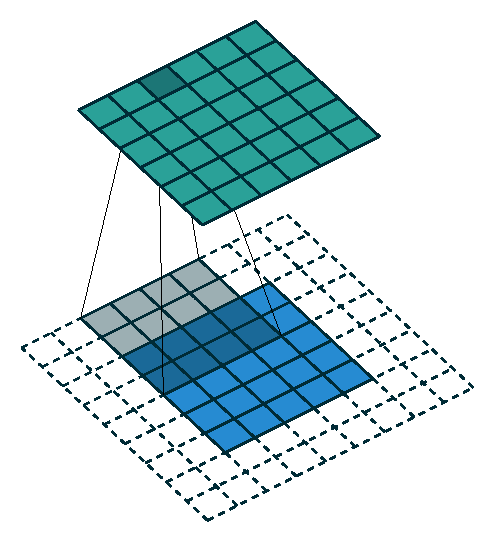
\includegraphics[width=0.24\textwidth]{pdf/arbitrary_padding_no_strides_02.pdf}
    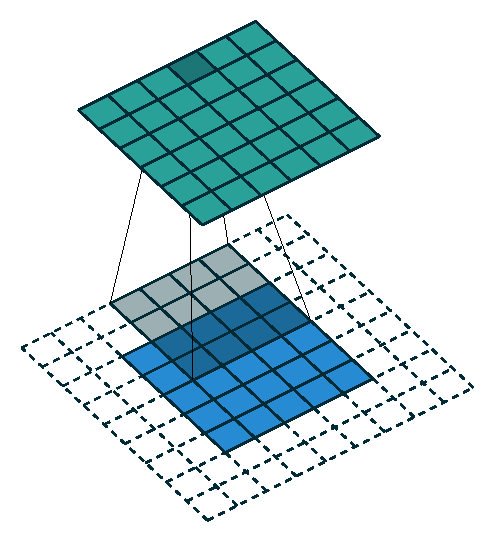
\includegraphics[width=0.24\textwidth]{pdf/arbitrary_padding_no_strides_03.pdf}
    \caption{\label{fig:arbitrary_padding_no_strides} Convolving a $4 \times 4$
        kernel over a $5 \times 5$ input padded with a $2 \times 2$ border of
        zeros using unit strides (i.e. $i = 5$, $k = 4$, $s = 1$ and $p = 2$).}
\end{figure}

\begin{figure}[p]
    \centering
    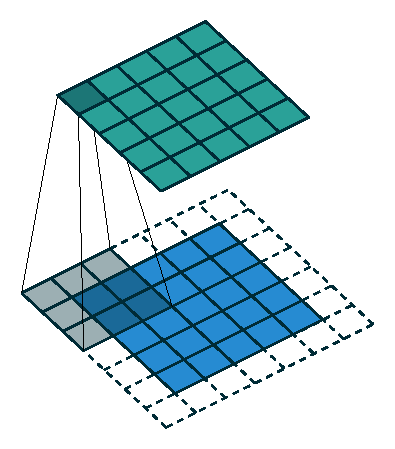
\includegraphics[width=0.24\textwidth]{pdf/same_padding_no_strides_00.pdf}
    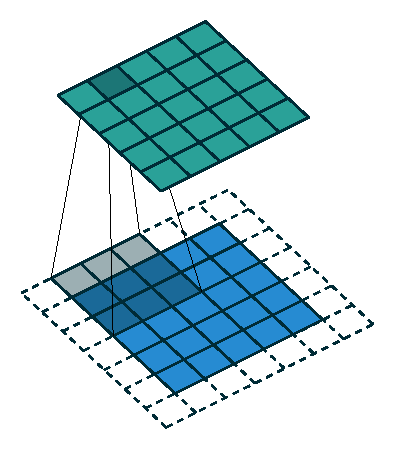
\includegraphics[width=0.24\textwidth]{pdf/same_padding_no_strides_01.pdf}
    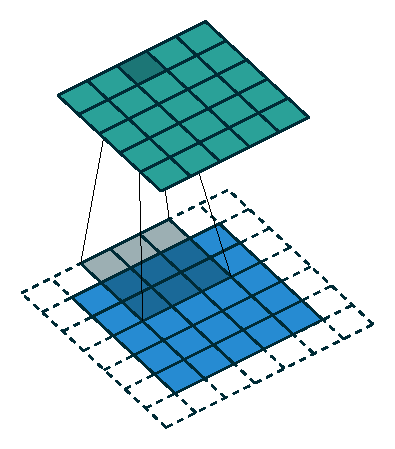
\includegraphics[width=0.24\textwidth]{pdf/same_padding_no_strides_02.pdf}
    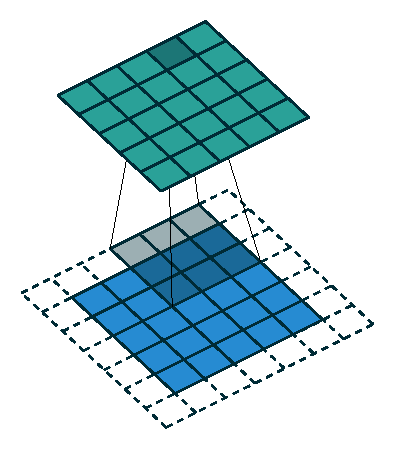
\includegraphics[width=0.24\textwidth]{pdf/same_padding_no_strides_03.pdf}
    \caption{\label{fig:same_padding_no_strides} Convolving a $3 \times 3$
        kernel over a $5 \times 5$ input using half padding and unit strides
        (i.e. $i = 5$, $k = 3$, $s = 1$ and $p = 1$).}
\end{figure}

\begin{figure}[p]
    \centering
    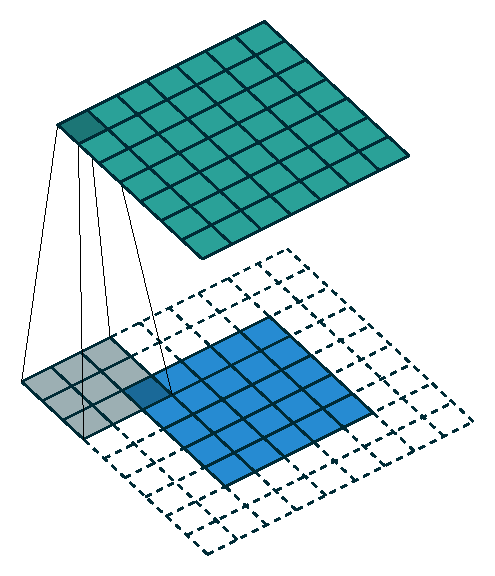
\includegraphics[width=0.24\textwidth]{pdf/full_padding_no_strides_00.pdf}
    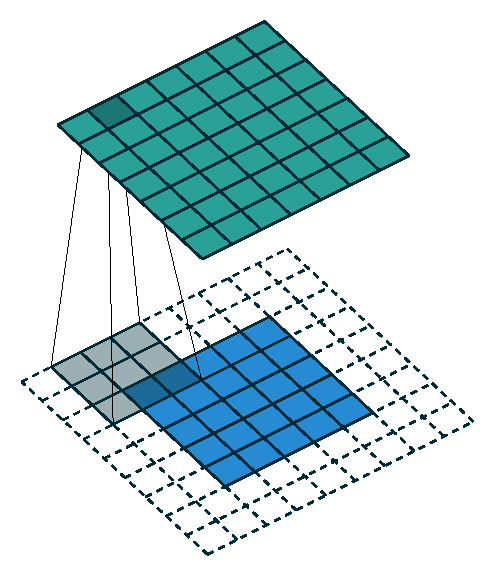
\includegraphics[width=0.24\textwidth]{pdf/full_padding_no_strides_01.pdf}
    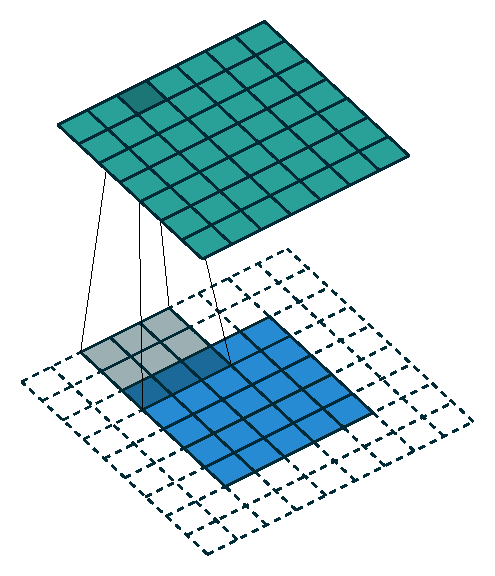
\includegraphics[width=0.24\textwidth]{pdf/full_padding_no_strides_02.pdf}
    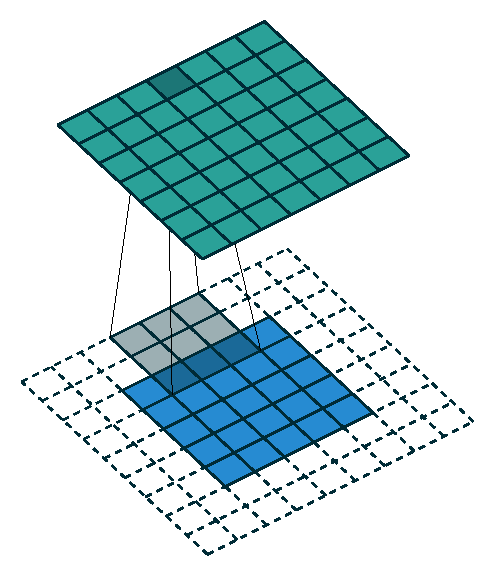
\includegraphics[width=0.24\textwidth]{pdf/full_padding_no_strides_03.pdf}
    \caption{\label{fig:full_padding_no_strides} Convolving a $3 \times 3$
        kernel over a $5 \times 5$ input using full padding and unit strides
        (i.e. $i = 5$, $k = 3$, $s = 1$ and $p = 2$).}
\end{figure}

\begin{figure}[p]
    \centering
    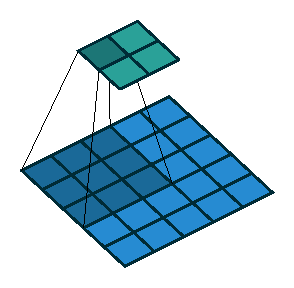
\includegraphics[width=0.24\textwidth]{pdf/no_padding_strides_00.pdf}
    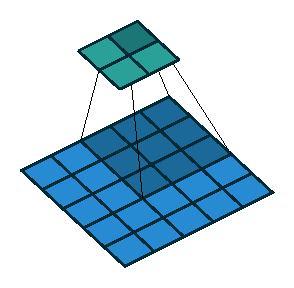
\includegraphics[width=0.24\textwidth]{pdf/no_padding_strides_01.pdf}
    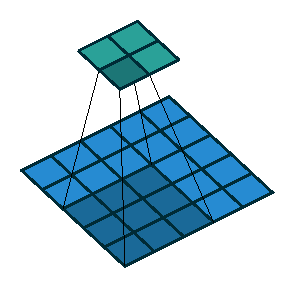
\includegraphics[width=0.24\textwidth]{pdf/no_padding_strides_02.pdf}
    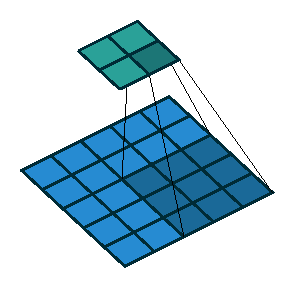
\includegraphics[width=0.24\textwidth]{pdf/no_padding_strides_03.pdf}
    \caption{\label{fig:no_padding_strides} Convolving a $3 \times 3$
        kernel over a $5 \times 5$ input using $2 \times 2$ strides (i.e.
        $i = 5$, $k = 3$, $s = 2$ and $p = 0$).}
\end{figure}

\begin{figure}[p]
    \centering
    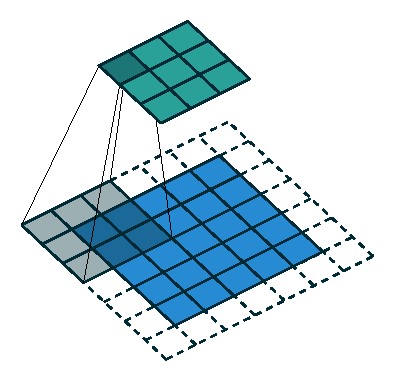
\includegraphics[width=0.24\textwidth]{pdf/padding_strides_00.pdf}
    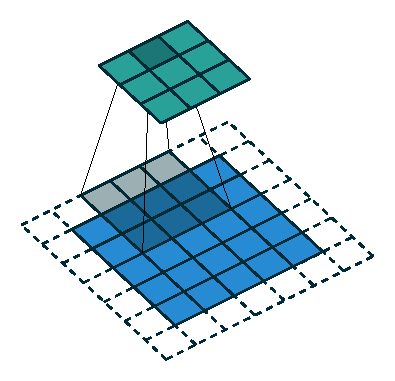
\includegraphics[width=0.24\textwidth]{pdf/padding_strides_01.pdf}
    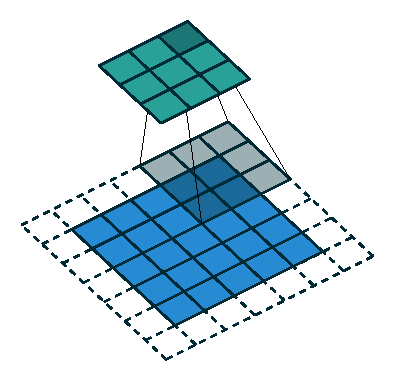
\includegraphics[width=0.24\textwidth]{pdf/padding_strides_02.pdf}
    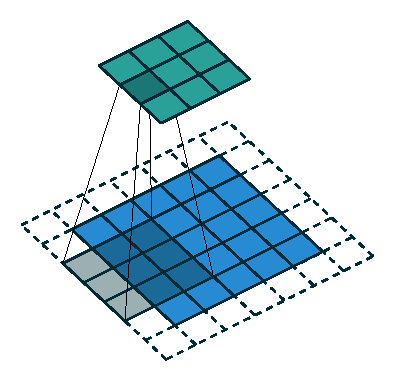
\includegraphics[width=0.24\textwidth]{pdf/padding_strides_03.pdf}
    \caption{\label{fig:padding_strides} Convolving a $3 \times 3$ kernel over a
        $5 \times 5$ input padded with a $1 \times 1$ border of zeros using $2
        \times 2$ strides (i.e.  $i = 5$, $k = 3$, $s = 2$ and $p = 1$).}
\end{figure}

\begin{figure}[p]
    \centering
    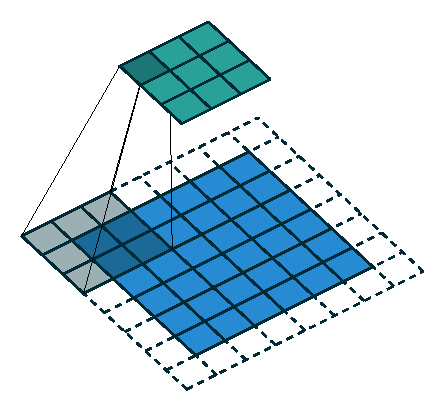
\includegraphics[width=0.24\textwidth]{pdf/padding_strides_odd_00.pdf}
    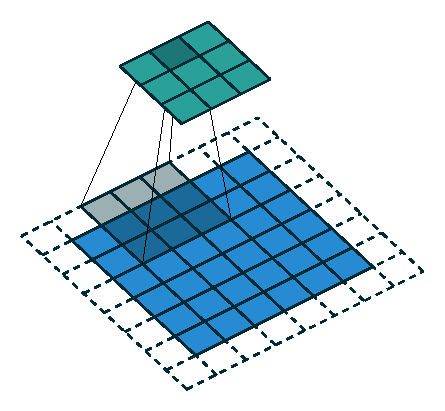
\includegraphics[width=0.24\textwidth]{pdf/padding_strides_odd_01.pdf}
    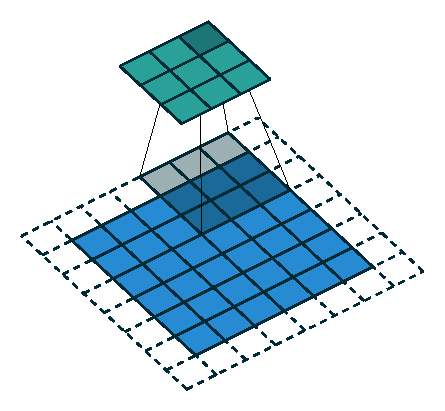
\includegraphics[width=0.24\textwidth]{pdf/padding_strides_odd_02.pdf}
    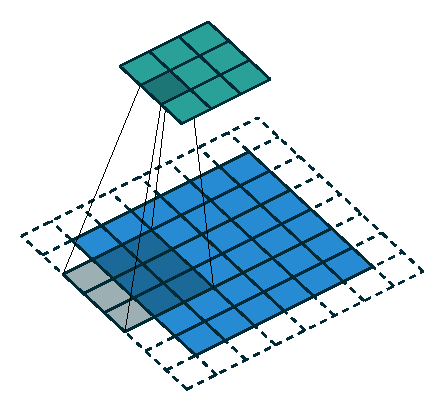
\includegraphics[width=0.24\textwidth]{pdf/padding_strides_odd_03.pdf}
    \caption{\label{fig:padding_strides_odd} Convolving a $3 \times 3$ kernel
        over a $6 \times 6$ input padded with a $1 \times 1$ border of zeros
        using $2 \times 2$ strides (i.e.  $i = 6$, $k = 3$, $s = 2$ and
        $p = 1$). In this case, the bottom row and right column of the
        zero-padded input are not covered by the kernel.}
\end{figure}

\begin{figure}[p]
    \centering
    \begin{subfigure}[t]{0.48\textwidth}
        \centering
        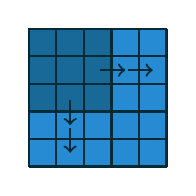
\begin{tikzpicture}[scale=.35,every node/.style={minimum size=1cm},
                            on grid]
            \draw[fill=blue] (0,0) rectangle (5,5);
            \draw[draw=base03, thick] (0,0) grid (5,5);
            \draw[fill=base02, opacity=0.4] (0,2) rectangle (3,5);
            \draw[step=10mm, base03, thick] (0,2) grid (3,5);
            \draw[draw=base03, ->, thick] (2.6,3.5) to  (3.5,3.5);
            \draw[draw=base03, ->, thick] (3.6,3.5) to  (4.5,3.5);
            \draw[draw=base03, ->, thick] (1.5,2.4) to  (1.5,1.5);
            \draw[draw=base03, ->, thick] (1.5,1.4) to  (1.5,0.5);
        \end{tikzpicture}
        \caption{\label{fig:no_padding_no_strides_explained} The kernel has to
            slide two steps to the right to touch the right side of the input
            and two steps downwards to touch the bottom side of the input.
            Adding one to account for the initial kernel position, the output
            size is $3 \times 3$.}
    \end{subfigure}
    ~
    \begin{subfigure}[t]{0.48\textwidth}
        \centering
        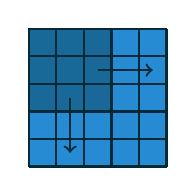
\begin{tikzpicture}[scale=.35,every node/.style={minimum size=1cm},
                            on grid]
            \draw[fill=blue] (0,0) rectangle (5,5);
            \draw[draw=base03, thick] (0,0) grid (5,5);
            \draw[fill=base02, opacity=0.4] (0,2) rectangle (3,5);
            \draw[step=10mm, base03, thick] (0,2) grid (3,5);
            \draw[draw=base03, ->, thick] (2.5,3.5) to  (4.5,3.5);
            \draw[draw=base03, ->, thick] (1.5,2.5) to  (1.5,0.5);
        \end{tikzpicture}
        \caption{\label{fig:no_padding_strides_explained} The kernel has to
            slide one step of size two to the right to touch the right side of
            the input and one step of size two downwards to touch the bottom
            side of the input. Adding one to account for the initial kernel
            position, the output size is $2 \times 2$.}
    \end{subfigure}
    \caption{Counting kernel positions.}
\end{figure}

\chapter{Transposed convolution arithmetic}

\section{Convolution vs. transposed convolution}

The need for transposed convolutions generally arises from the desire to use a
transformation going from something that has the output shape of some
convolution to something that has the input shape of the same convolution while
maintaining a connectivity pattern that is compatible with said convolution.
For instance, one might use such a transformation as the decoding layer of a
convolutional autoencoder in order to obtain a learned inverse of the encoding
convolution.

Once again, the convolutional case is considerably more complex than the
fully-connected case, which only requires to use a weight matrix whose shape has
been transposed. However, since every convolution boils down to an efficient
implementation of a matrix operation, the insights gained from the
fully-connected case are useful in solving the convolutional case.

Take for instance the convolution represented in
\autoref{fig:no_padding_no_strides}. If the input and output were to be unrolled
into vectors from left to right, top to bottom, the matrix representation of the
convolution would look like

\begin{equation*}
\resizebox{.98\hsize}{!}{$
    \begin{pmatrix}
    w_{0,0} & w_{0,1} & w_{0,2} & 0       & w_{1,0} & w_{1,1} & w_{1,2} & 0       &
    w_{2,0} & w_{2,1} & w_{2,2} & 0       & 0       & 0       & 0       & 0       \\
    0       & w_{0,0} & w_{0,1} & w_{0,2} & 0       & w_{1,0} & w_{1,1} & w_{1,2} &
    0       & w_{2,0} & w_{2,1} & w_{2,2} & 0       & 0       & 0       & 0       \\
    0       & 0       & 0       & 0       & w_{0,0} & w_{0,1} & w_{0,2} & 0       &
    w_{1,0} & w_{1,1} & w_{1,2} & 0       & w_{2,0} & w_{2,1} & w_{2,2} & 0       \\
    0       & 0       & 0       & 0       & 0       & w_{0,0} & w_{0,1} & w_{0,2} &
    0       & w_{1,0} & w_{1,1} & w_{1,2} & 0       & w_{2,0} & w_{2,1} & w_{2,2} \\
    \end{pmatrix}$}
\end{equation*}

where $w_{i,j}$ is the element of the kernel located at row $i$ and column $j$.
This linear operation takes a 16-dimensional vector as input and produces a
4-dimensional vector as output.

What would happen if this matrix was transposed and the values for $\mathbf{w}$
were replaced with the values of another $3 \times 3$ kernel $\mathbf{u}$? The
transformation would take a 4-dimensional vector as input and produce a
16-dimensional vector as output {\em while keeping a connectivity pattern
compatible with the convolution presented in
\autoref{fig:no_padding_no_strides}}. This is what is referred to as a {\em
transposed convolution}.

Note that if $\mathbf{w}$ is {\em not} replaced with $\mathbf{u}$, the resulting
operation is a direct transpose of the convolution defined by $\mathbf{w}$,
which is {\em exactly} what is needed for gradient backpropagation. In other
words, the transposed convolution operation can be thought of as the gradient of
{\em some} convolution with respect to its input.

The fortunate thing about transposed convolutions is that they are themselves
convolutions, albeit with some additional processing on the input.

This section will proceed somewhat backwards with respect to the convolution
arithmetic section. Case by case, the analysis will concentrate on how the
transpose of convolutions can be expressed in terms of convolutions.

\section{No zero-padding, unit strides, transposed}

\autoref{fig:no_padding_no_strides_transposed} shows the effect of applying the
transpose of the matrix above on a $4 \times 4$ input (i.e. $i = 4$, $k = 3$, $s
= 1$ and $p = 0$).

Note that although equivalent to the transposed matrix, this visualization adds
a lot of zero multiplications in the form of zero padding. This is done for
illustration purposes, but it is inefficient, and software implementations will
normally not perform the useless zero multiplications.

The transposed convolution is equivalent to convolving a $3 \times 3$ kernel
over a $2 \times 2$ input padded with a $2 \times 2$ border of zeros using unit
strides (i.e. $i' = 2$, $k' = k$, $s' = 1$ and $p' = 2$). The kernel size and
stride remain the same, but the input to the transposed convolution is now
zero-padded.

One way to understand the logic behind zero padding is to consider what would be
necessary to produce a transposed convolution with the same connectivity pattern
as its converse convolution.

In particular, the corner pixels of the input only contribute to the corner
pixels of the output: the top left input pixel is only connected to the top left
output pixel, the top right pixel is only connected to the top right output
pixel, and so on. This is achieved by zero padding the input such that the
kernel only touches a corner pixel when it is in the associated corner position.

These observations give rise to the following property:

\begin{prop}\label{prop:no_padding_no_strides_transposed}
A convolution described by $k$, $s = 1$ and $p = 0$ has an associated transposed
convolution described by $k' = k$, $s' = 1$ and $p' = k - 1$ and its output size
is
\begin{equation*}
    o' = i' + (k - 1).
\end{equation*}
\end{prop}

Note that this corresponds to a fully padded convolution with unit strides on
the transposed convolution's input.

\section{Zero padding, unit strides, transposed}

Knowing that the transpose of a non-padded convolution involves convolving a
zero-padded input, it would be reasonable to assume that the transpose of a
zero-padded convolution involves convolving an input padded with {\em less}
zeros.

\autoref{fig:arbitrary_padding_no_strides_transposed} shows that it is indeed
the case by providing an example for $i = 5$, $k = 4$ and $p = 2$.

The following property applies for zero-padded convolutions:

\begin{prop}\label{prop:arbitrary_padding_no_strides_transposed}
A convolution described by $k$, $s = 1$ and $p$ has an associated transposed
convolution described by $k' = k$, $s' = 1$ and $p' = k - p - 1$ and its output
size is
\begin{equation*}
    o' = i' + (k - 1) - 2p.
\end{equation*}
\end{prop}

The transposes of convolutions with half and full padding have elegant
properties.

\subsection{Half padding, transposed}

Knowing that a half padded convolution produces an output with the same size as
the input, it is unsurprising that the transpose of a half padded convolution
is itself a half padded convolution:

\begin{prop}\label{prop:half_padding_no_strides_transposed}
A convolution described by $k = 2n + 1, \quad n \in \mathbb{N}$, $s = 1$ and $p
= \lfloor k / 2 \rfloor = n$ has an associated transposed convolution described
by $k' = k$, $s' = 1$ and $p' = \lfloor k / 2 \rfloor$ and its output size is
\begin{equation*}
\begin{split}
    o' &= i' + (k - 1) - 2p \\
       &= i' + 2n - 2n \\
       &= i'.
\end{split}
\end{equation*}
\end{prop}

\autoref{fig:same_padding_no_strides_transposed} provides an example for $i =
5$, $k = 3$ and (therefore) $p = 1$.

\subsection{Full padding, transposed}

Knowing that a non-padded convolution has a transpose which involves full
padding, it is also unsurprising that the transpose of a fully padded
convolution is a non-padded convolution:

\begin{prop}\label{prop:full_padding_no_strides_transposed}
A convolution described by $k$, $s = 1$ and $p = k - 1$ has an associated
transposed convolution described by $k' = k$, $s' = 1$ and $p' = 0$ and its
output size is
\begin{equation*}
\begin{split}
    o' &= i' + (k - 1) - 2p \\
       &= i' - (k - 1)
\end{split}
\end{equation*}
\end{prop}

\autoref{fig:full_padding_no_strides_transposed} provides an example for $i =
5$, $k = 3$ and (therefore) $p = 2$.

\section{No zero-padding, non-unit strides, transposed}

Using the same kind of deductive logic as for zero-padded convolutions, one
might expect that the transpose of a convolution with $s > 1$ involves a
convolution with $s < 1$. As will be explained, this is a valid intuition, which
is why transposed convolutions have sometimes been called {\em fractionally
strided convolutions}.

\autoref{fig:no_padding_strides_transposed} provides an example for $i = 5$, $k
= 3$ and $s = 2$ which helps understand what fractional strides involve: zeros
are inserted {\em between} input units, which makes the kernel move around at a
slower pace than with unit strides.

Doing so is inefficient and real-world implementations avoid useless
multiplications by zero, but conceptually it is how the transpose of a strided
convolution can be thought of.

For the moment, it will be assumed that the convolution is non-padded ($p = 0$)
and that its input size $i$ is such that $i - k$ is a multiple of $s$. In that
case, the following property holds:

\begin{prop}\label{prop:no_padding_strides_transposed}
A convolution described by $k$, $s$ and $p = 0$ and whose input size is such
that $i - k$ is a multiple of $s$ has an associated transposed convolution
described by $\tilde{i}'$, $k' = k$, $s' = 1$ and $p' = k - 1$, where
$\tilde{i}'$ is the size of the stretched input obtained by adding $s - 1$ zeros
between each input unit, and its output size is
\begin{equation*}
\begin{split}
    o' = s (i' - 1) + k.
\end{split}
\end{equation*}
\end{prop}

\section{Zero-padding, non-unit strides, transposed}

Still assuming that the convolution's input size $i$ is such that $i - k$ is a
multiple of $s$, the analysis is extended to the zero-padded case by combining
\autoref{prop:arbitrary_padding_no_strides_transposed} and
\autoref{prop:no_padding_strides_transposed}:

\begin{prop}\label{prop:padding_strides_transposed}
A convolution described by $k$, $s$ and $p$ and whose input size is such
that $i - k$ is a multiple of $s$ has an associated transposed convolution
described by $\tilde{i}'$, $k' = k$, $s' = 1$ and $p' = k - p - 1$, where
$\tilde{i}'$ is the size of the stretched input obtained by adding $s - 1$ zeros
between each input unit, and its output size is
\begin{equation*}
\begin{split}
    o' = s (i' - 1) + k - 2p.
\end{split}
\end{equation*}
\end{prop}

\autoref{fig:padding_strides_transposed} provides an example for $i = 5$, $k =
3$, $s = 2$ and $p = 1$.

The assumption that $i$ is such that $i - k$ is a multiple of $s$ is relaxed by
introducing another parameter $a \in \{0, \ldots, s - 1\}$ that allows to
distinguish between the $s$ different cases leading to $i'$:

\begin{prop}\label{prop:padding_strides_transposed_odd}
A convolution described by $k$, $s$ and $p$, with $a = \mod s$,
has an associated transposed convolution described by $a$, $\tilde{i}'$,
$k' = k$, $s' = 1$ and $p' = k - p - 1$, where
$\tilde{i}'$ is the size of the stretched input obtained by adding $s - 1$ zeros
between each input unit, and $a = (i + 2p - k) \mod s$ represents the number of
zeros added to the right and bottom edge of the input, and its output size is
\begin{equation*}
\begin{split}
    o' = s (i' - 1) + a + k - 2p.
\end{split}
\end{equation*}
\end{prop}

\autoref{fig:padding_strides_odd_transposed} provides an example for $i = 6$, $k
= 3$, $s = 2$ and $p = 1$.

\begin{figure}[p]
    \centering
    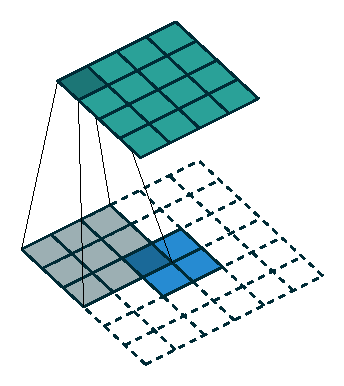
\includegraphics[width=0.24\textwidth]{pdf/no_padding_no_strides_transposed_00.pdf}
    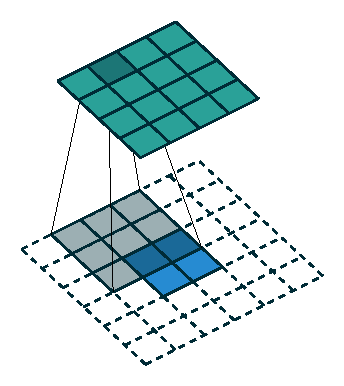
\includegraphics[width=0.24\textwidth]{pdf/no_padding_no_strides_transposed_01.pdf}
    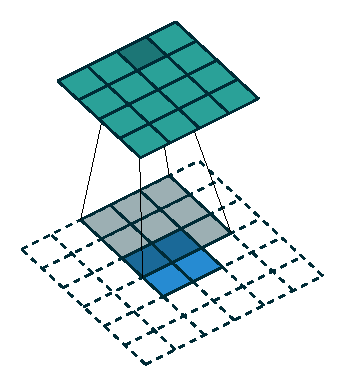
\includegraphics[width=0.24\textwidth]{pdf/no_padding_no_strides_transposed_02.pdf}
    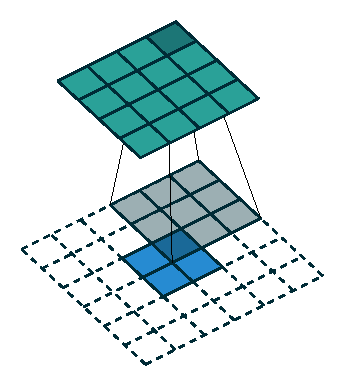
\includegraphics[width=0.24\textwidth]{pdf/no_padding_no_strides_transposed_03.pdf}
    \caption{\label{fig:no_padding_no_strides_transposed} The transpose of
        convolving a $3 \times 3$ kernel over a $4 \times 4$ input using unit
        strides (i.e. $i = 4$, $k = 3$, $s = 1$ and $p = 0$) is equivalent to
        convolving a $3 \times 3$ kernel over a $2 \times 2$ input padded with
        a $2 \times 2$ border of zeros using unit strides (i.e. $i' = 2$, $k' =
        k$, $s' = 1$ and $p' = 2$).}
\end{figure}

\begin{figure}[p]
    \centering
    \includegraphics[width=0.24\textwidth]{pdf/arbitrary_padding_no_strides_transposed_00.pdf}
    \includegraphics[width=0.24\textwidth]{pdf/arbitrary_padding_no_strides_transposed_01.pdf}
    \includegraphics[width=0.24\textwidth]{pdf/arbitrary_padding_no_strides_transposed_02.pdf}
    \includegraphics[width=0.24\textwidth]{pdf/arbitrary_padding_no_strides_transposed_03.pdf}
    \caption{\label{fig:arbitrary_padding_no_strides_transposed} The transpose
        of convolving a $4 \times 4$ kernel over a $5 \times 5$ input padded
        with a $2 \times 2$ border of zeros using unit strides (i.e. $i = 5$,
        $k = 4$, $s = 1$ and $p = 2$) is equivalent to convolving a $4 \times 4$
        kernel over a $6 \times 6$ input padded with a $1 \times 1$ border of
        zeros using unit strides (i.e. $i' = 6$, $k' = k$, $s' = 1$ and $p' =
        1$).}
\end{figure}

\begin{figure}[p]
    \centering
    \includegraphics[width=0.24\textwidth]{pdf/same_padding_no_strides_transposed_00.pdf}
    \includegraphics[width=0.24\textwidth]{pdf/same_padding_no_strides_transposed_01.pdf}
    \includegraphics[width=0.24\textwidth]{pdf/same_padding_no_strides_transposed_02.pdf}
    \includegraphics[width=0.24\textwidth]{pdf/same_padding_no_strides_transposed_03.pdf}
    \caption{\label{fig:same_padding_no_strides_transposed} The transpose
        of convolving a $3 \times 3$ kernel over a $5 \times 5$ input using half
        padding and unit strides (i.e. $i = 5$, $k = 3$, $s = 1$ and $p = 1$) is
        equivalent to convolving a $3 \times 3$ kernel over a $5 \times 5$ input
        using half padding and unit strides (i.e. $i' = 5$, $k' = k$, $s' = 1$
        and $p' = 1$).}
\end{figure}

\begin{figure}[p]
    \centering
    \includegraphics[width=0.24\textwidth]{pdf/full_padding_no_strides_transposed_00.pdf}
    \includegraphics[width=0.24\textwidth]{pdf/full_padding_no_strides_transposed_01.pdf}
    \includegraphics[width=0.24\textwidth]{pdf/full_padding_no_strides_transposed_02.pdf}
    \includegraphics[width=0.24\textwidth]{pdf/full_padding_no_strides_transposed_03.pdf}
    \caption{\label{fig:full_padding_no_strides_transposed} The transpose
        of convolving a $3 \times 3$ kernel over a $5 \times 5$ input using full
        padding and unit strides (i.e. $i = 5$, $k = 3$, $s = 1$ and $p = 2$) is
        equivalent to convolving a $3 \times 3$ kernel over a $7 \times 7$ input
        using unit strides (i.e. $i' = 7$, $k' = k$, $s' = 1$ and $p' = 0$).}
\end{figure}

\begin{figure}[p]
    \centering
    \includegraphics[width=0.24\textwidth]{pdf/no_padding_strides_transposed_00.pdf}
    \includegraphics[width=0.24\textwidth]{pdf/no_padding_strides_transposed_01.pdf}
    \includegraphics[width=0.24\textwidth]{pdf/no_padding_strides_transposed_02.pdf}
    \includegraphics[width=0.24\textwidth]{pdf/no_padding_strides_transposed_03.pdf}
    \caption{\label{fig:no_padding_strides_transposed} The transpose of
        convolving a $3 \times 3$ kernel over a $5 \times 5$ input using $2
        \times 2$ strides (i.e. $i = 5$, $k = 3$, $s = 2$ and $p = 0$) is
        equivalent to convolving a $3 \times 3$ kernel over a $2 \times 2$ input
        padded with a $2 \times 2$ border of zeros with $1$ zero inserted
        between inputs using unit strides (i.e. $i' = 2$, $\tilde{i}' = 3$, $k'
        = k$, $s' = 1$ and $p' = 2$).}
\end{figure}

\begin{figure}[p]
    \centering
    \includegraphics[width=0.24\textwidth]{pdf/padding_strides_transposed_00.pdf}
    \includegraphics[width=0.24\textwidth]{pdf/padding_strides_transposed_01.pdf}
    \includegraphics[width=0.24\textwidth]{pdf/padding_strides_transposed_02.pdf}
    \includegraphics[width=0.24\textwidth]{pdf/padding_strides_transposed_03.pdf}
    \caption{\label{fig:padding_strides_transposed} The transpose of convolving
        a $3 \times 3$ kernel over a $5 \times 5$ input padded with a $1 \times
        1$ border of zeros using $2 \times 2$ strides (i.e. $i = 5$, $k = 3$, $s
        = 2$ and $p = 1$) is equivalent to convolving a $3 \times 3$ kernel over
        a $2 \times 2$ input padded with a $1 \times 1$ border of zeros with $1$
        zero inserted between inputs using unit strides (i.e. $i' = 2$,
        $\tilde{i}' = 3$, $k' = k$, $s' = 1$ and $p' = 1$).}
\end{figure}

\begin{figure}[p]
    \centering
    \includegraphics[width=0.24\textwidth]{pdf/padding_strides_odd_transposed_00.pdf}
    \includegraphics[width=0.24\textwidth]{pdf/padding_strides_odd_transposed_01.pdf}
    \includegraphics[width=0.24\textwidth]{pdf/padding_strides_odd_transposed_02.pdf}
    \includegraphics[width=0.24\textwidth]{pdf/padding_strides_odd_transposed_03.pdf}
    \caption{\label{fig:padding_strides_odd_transposed} \todo{FIXME} The
        transpose of convolving a $3 \times 3$ kernel over a $6 \times 6$ input
        padded with a $1 \times 1$ border of zeros using $2 \times 2$ strides
        (i.e. $i = 6$, $k = 3$, $s = 2$ and $p = 1$) is equivalent to convolving
        a $3 \times 3$ kernel over a $2 \times 2$ input padded with a $1 \times
        1$ border of zeros with $1$ zero inserted between inputs using unit
        strides (i.e. $i' = 2$, $\tilde{i}' = 3$, $a = 1$, $k' = k$, $s' = 1$
        and $p' = 1$).}
\end{figure}

\bibliography{bibliography}
\bibliographystyle{natbib}
\end{document}
